% Springer
%\documentclass[smallextended]{svjour3}  

%Standard Article
%\documentclass[10pt,twoside=true, twocolumn]{article}

% KOMA Article
\documentclass[BCOR=1mm, DIV=calc,10pt,
twoside=true,
twocolumn,
headings=normal]{scrartcl}
%\KOMAoptions{DIV=calc}% recalculate the page layout with a calculated DIV value

% Recommended, but optional, packages for figures and better typesetting:
\usepackage{microtype}
\usepackage{graphicx}
%\usepackage{subfigure}
\usepackage{booktabs} % for professional tables

\usepackage{amsmath}
\usepackage{bm}
\usepackage{url}

% Attempt to make hyperref and algorithmic work together better:
\newcommand{\theHalgorithm}{\arabic{algorithm}}

\usepackage{cite}
\usepackage{amsmath,amssymb,amsfonts}
%\usepackage{algorithmic}
\usepackage{graphicx}
\usepackage{textcomp}
\usepackage{xcolor}

\usepackage{authblk}


\newcommand{\fig}{Fig.}
\newcommand{\eqn}{Eqn.}
\newcommand{\tab}{Tab.}
\newcommand{\wrt}{w.r.t.}
\newcommand{\etal}{ {\em et al.}}


\begin{document}


\title{Demand Forecasting of individual Probability Density Functions with Machine Learning}

%Springer
%\author{
%\underline{Felix Wick} \and
%Ulrich Kerzel \and
%Martin Hahn \and
%Moritz Wolf \and
%Trapti Singhal \and
%Michael Feindt}
%
%\institute{ 
%F. Wick (corresponding author) \at 
%Blue Yonder GmbH \\ \email{felix.wick@blueyonder.com}
%\and
%U. Kerzel \at 
%IUBH Internationale Hochschule \\ \email{u.kerzel@iubh-fernstudium.de}
%\and
%M. Hahn \at
%Blue Yonder GmbH \\ \email{martin.hahn@blueyonder.com}
%\and
%M. Wolf \at 
%Blue Yonder GmbH \\ \email{moritz.wolf@blueyonder.com}
%\and
%T. Singhal \at
%Blue Yonder India Private Limited \\ \email{trapti.singhal@blueyonder.com}
%\and
%M. Feindt \at
%Blue Yonder GmbH \\ \email{michael.feindt@blueyonder.com}
%}



\author[1]{Felix Wick } %\thanks{felix.wick@blueyonder.com}}
\author[3]{Ulrich Kerzel }%\thanks{u.kerzel@iubh-fernstudium.de}}
\author[1]{Martin Hahn }%\thanks{martin.hahn@blueyonder.com}}
\author[1]{Moritz Wolf }%\thanks{moritz.wolf@blueyonder.com}}
\author[2]{Trapti Singhal }%\thanks{trapti.singhal@blueyonder.com}}
\author[1]{Michael Feindt }%\thanks{michael.feindt@blueyonder.com}}
\affil[1]{\small Blue Yonder GmbH (Ohiostra{\ss}e 8, 76149 Karlsruhe, Germany)}
\affil[2]{\small Blue Yonder India Private Limited (Bengaluru, India)}
\affil[3]{\small IUBH Internationale Hochschule (Erfurt, Germany)}


\date{}
% Springer
%\titlerunning{Demand Forecasting as a Probability Distribution}
%\authorrunning{F. Wick et al.}

\maketitle

\begin{abstract}
Demand forecasting is a central component for many aspects of supply chain operations, as it provides crucial input for subsequent decision making like ordering processes. While machine learning methods can significantly improve prediction accuracy over traditional time series forecasting, the calculated predictions are often just point estimations for the conditional mean of the underlying probability distribution, and the most powerful approaches, like deep learning, are usually opaque in terms of how its individual predictions can be interpreted. Using the novel supervised machine learning method ``Cyclic Boosting'', complete individual probability density functions can be predicted instead of single numbers. While metrics evaluating point estimates are widely used, methods for assessing the accuracy of predicted distributions are rare and this work proposes new techniques for both qualitative and quantitative evaluation methods. Additionally, each single prediction obtained with this framework is explainable. This is a major benefit in particular for practitioners, as this allows them to avoid ``black-box'' models and understand the contributing factors for each individual prediction. 
\end{abstract}

{Keywords: \textbf{explainable machine learning, demand forecasting, probability distribution}}
%Springer
%\keywords{explainable machine learning \and demand forecasting \and probability distribution \and quantile plot}

\section{Introduction}
\label{sec:intro}

Demand forecasting is one of the main challenges for retailers and is at the core of supply chain business operations. Due to its stochastic nature, demand is difficult to forecast: It depends on many influencing factors and can be interpreted as a random variable that is described by an appropriate probability density function (PDF). Demand estimation is further complicated by the fact that retailers typically only observe realized sales rather than the actual demand, and, in case the demand exceeds the current stock level, the data become censored. Demand forecasting is an application of time series forecasting and it is important to note that demand as a random variable is not identically and independently distributed (i.i.d.) between different items and sales locations. While the probability distribution describing the demand can be attributed to a given family or parameterization, the exact parameters vary: Seasonal effects, finite life cycles of products, and the introduction of new products influence the demand distribution, as well as the local weather at the retail location or the retail location itself in terms of size, assortment range, customer diversity, and other factors. The retailers themselves also actively influence demand by using advertisements to highlight products, offering rebates or discounts for specific products, as well as pursuing an active pricing strategy. This means that while we can generally assume that demand follows a specific type of probability distribution, its parameters are unique to the instance for which an estimate is required. For example, the probability distribution governing the demand of a particular item is specific to the item, date, and retail location for which the forecast is made, and depends on a wide range of further influencing factors.

Because of the access to  Big Data, a vast amount of these data associated with demand, such as historic sales records, information about promotional events or advertisements, pricing information, local weather at retail locations, seasonal information, as well as many further variables, can be captured, stored, and processed. Different methods, such as traditional univariate time series forecasting or modern supervised machine learning algorithms, can then be used to predict the demand distribution for individual products sold at specific locations, corrected for censored data. Demand forecasting for retailers often requires to predict millions of item-store combinations daily, and traditional univariate time series forecasting methods operate on each of these many individual time series separately. Machine learning, on the contrary, optimizes all individual time series together, improving the generalizability of the method by exploiting common aspects between them. This leads to a drastic reduction in variance of the model, and in turn to an improvement of the forecast quality of each of the individual time series. Furthermore, machine learning enables a natural way to include the many exogenous variables influencing demand as features of the model, what reduces also the bias compared to traditional time series forecasting approaches which mainly rely on the historic sales.

In order to make operational decisions, an optimal demand point estimator has to be defined, that can be used to derive ordering decisions in the replenishment process of the retailer. The ordering decision process is complicated by a range of factors: Even in the case of perfect demand forecasts, the decision maker has to consider lot sizes defined by the wholesaler or manufacturer as well as to balance conflicting metrics to reach an optimal decision. Ordering too few items may result in out of stock situations leading to unrealized demand and unsatisfied customers. Ordering too many items results in excess inventory, which increases transport and storage costs and, in the case of perishable goods, excessive waste, as spoiled items need to be disposed of at additional cost and potentially even environmental impact. This situation is particularly noticeable in the so called ``ultra-fresh'' category, which includes items such as bakery products, ready-meals, fresh dairy products, or certain meat products such as ground meat. These items typically have a shelf-life ranging from less than a business day to a few business days at most, with a continuous spectrum in between, depending on the exact item. In many situations, additional constraints have to be considered to reach an optimal ordering decision: Delivery cycles of items may vary depending on the type of item and the wholesaler or manufacturer from which they are procured. Retailers also operate at a given service level to guarantee that a certain level of demand can be fulfilled. The exact service level typically depends on the overall business policy of the retailer and may also depend on individual products, ranging from ``never-out-of-stock'' items to a service level exceeding, e.g., 90 percent. Therefore, demand forecasts are ideally made in the form of full individual probability density distributions, from which optimal point estimators can be derived, which in turn serve as starting point to determine the subsequent ordering decisions.

The remainder of the paper is organized as follows: We first review the relevant literature and existing work in sec. \ref{sec:LitRev}. We then describe our method to predict individual negative binomial PDFs by means of a parametric approach including two distinct machine learning models for mean of variance in sec. \ref{sec:pdfEstimation}. After that, we describe novel techniques for the qualitative and quantitative evaluation of PDF predictions in sec. \ref{sec:pdfEvaluation}. And finally, we present a demand forecasting example to show an application of our methods in sec. \ref{sec:example}.


\section{Literature Review}
\label{sec:LitRev}

Inventory management offers a rich theory and the extensive body of research can be broadly grouped into two categories, where the inventory control problem is either based on some knowledge of the underlying demand distribution or an integrated approach that seeks to map directly from the observed data to the ordering decision. More traditional inventory control systems rely on the knowledge of the demand distribution in one form or another, see e.g. \cite{silver1998} for an overview. In $(s,S)$ type inventory control systems \cite{Scarf1958}, inventory levels are monitored at regular intervals and orders are dispatched once the inventory level reaches a minimal value $s$. In case of linear holding and shortage costs, such policies are optimal \cite{Scarf1959}, although perishable goods pose more challenges, see e.g. \cite{Nahmias1973,Nahmias1975,nahmias1978}. Additionally, service level constraints can be included in these kind of inventory control systems \cite{minner2010periodic}. Perishable goods are well described by the ``newsvendor problem'' \cite{Edgeworth}, where, in the simplest case, all stock perishes at the end of the selling period (e.g. a business day). For a detailed review of the newsvendor problem see e.g. \cite{Khouja1999537}. Assuming linear underage and overage costs $b,h >0$, the optimal quantile $q_{\mathrm{opt}} = {b}/{(b+h})$ of a known demand distribution $f(D)$ can be calculated exactly. However, it should be noted that demand is not independent between different samples for a given date. For example, a promotion applied to one product can affect the sales of related products within the assortment. This implies that the demand forecasts for multiple items or a given assortment range cannot be treated as individual newsvendor-type predictions but need to be modeled holistically.

The direct approach is often referred to as ``data-driven newsvendor'' and discussed e.g. in \cite{beutel2012safety,ban2019big,bertsimas2020predictive,oroojlooyjadid2020applying}. It aims to avoid estimating the underlying probability distribution for demand and use the available data (historic sales records and further variables) to derive the operational decisions (i.e., the order quantity) directly. An overview of a range of different approaches can also be found in \cite{huber2019data}. Although the integrated approach seems preferable at first glance, since it avoids determining the full demand distribution and results directly in the desired operational decision, the indirect approach via demand forecasts offers some substantial advantages. First, demand forecasts in form of full PDFs can be used to simulate the performance of the relevant metrics on the level of individual item, and, for example, optimize the impact on business strategy decisions on conflicting metrics such as out of stock (i.e., lost sales) and waste rate. From a practitioners perspective, separating the demand forecast from the operational decisions (i.e., calculating the order quantities for the next delivery cycle) enables longer-term planning and reduces the complexity, as it avoids coupling delivery schedules of multiple wholesalers and manufacturers with the forecast of customer demand. It also allows to share long-term demand predictions with other business units or external vendors and wholesalers to ease their planning for the production and supply chain processes upstream of the retailer. From the perspective of the industrial practice of a vendor of supply chain methods and tools, modeling the demand separately from deriving the subsequent orders has the additional benefit that multiple retail chains can benefit from any improvement in the model description, even if the specific retailers are unrelated to each other. Additionally, a purely data-driven approach going from the observed data directly to the operational decision (such as the order quantity) does not allow to analyze the data-generating process, i.e., the mechanism behind the stochastic behavior of the customer demand. This is crucial, for example, if a causal analysis is planned, such as a study of the effect of promotions, advertisements, price changes, or other demand shaping factors in either Pearl's do-calculus \cite{PearlCausality} or Rubin's potential outcomes framework \cite{rubin1974estimating}. Using an operational quantity such as the order quantity will in most cases act as an insufficient proxy for the quantity of interest (customer demand) and likely lead to unnecessary causal pathways that one may not be able to fully control for.

Therefore, the main objective in solving the inventory control problem is to determine the underlying demand distribution. The simplest approach is to use the observed sales records and forecast these via sample average approximation (SAA), see, e.g., \cite{shapiro2014} for an overview, or as a time series (see, e.g., \cite{alwan2016}), for example by means of auto-regressive integrated moving average (ARIMA) \cite{BoxJenkins}, exponential smoothing \cite{ExponentialSmoothing}, or structural time series models \cite{StructuralTS}. However, these approaches do not make use of any data apart from the sales records themselves, although we know that many variables such as price, advertisements,  weather influence, and others are highly correlated with the demand. Saghafian and Tomlin \cite{saghafian2016newsvendor} propose to include partial information about the distribution in the derivation of the operational decision, i.e., the calculation of the optimal order quantity. As described in sec. \ref{sec:intro}, modern supervised machine learning techniques can overcome many of the issues of the more traditional approaches, and therefore are the method of choice in most use cases today (see, e.g., \cite{tsforecasting,ZHANG199835,rnn,transformer}).

In order to be able to fully optimize the operational decision, it is critical to reconstruct a full demand distribution. This also implies that a simple point-estimator, as provided by the most common statistical techniques and machine learning approaches, will not suffice. Instead, we need to determine the full demand distribution from data, conditional on the relevant variables such as date, location, and item, taking all auxiliary data such as article characteristics, pricing, advertisements, retail location details, etc. into account. This can be done in several ways: Quantile regression \cite{koenker2001,wen2017} can be implemented in various frameworks and used to estimate a range of quantiles for each predicted distribution, from which an empirical probability distribution can be interpolated. Using a dedicated neural network \cite{Feindt2006190}, either the full PDF or a defined range of quantiles can be calculated directly from the data for each individual prediction without assuming an underlying model. Alternatively, one can assume a given demand model and fit the model parameters instead of reconstructing the complete distribution \cite{astonpr373, SALINAS20201181}. This approach is computationally favorable and usually more robust, as fewer parameters need to be estimated. Empirically, one can determine the best fitting distribution from data \cite{adan1995}. However, given the stochastic nature of the demand, such an empirically determined distribution is not expected to be stable and prone to sudden changes. Instead, the choice of the demand distribution should be motivated by theoretic considerations. The discrete demand is typically modeled as a negative binomial distribution (NBD), also known as Gamma-Poisson distribution \cite{Ehrenberg1959,Ehrenberg1967,Ehrenberg1972,Chatfield1973,Schmittlein_1985}. This distribution arises if the Poisson parameter $\mu$ is a random variable itself, which follows a Gamma distribution. The NBD has two parameters, $\mu$ and $ \sigma^2 > \mu$, and is over-dispersed compared to the Poisson distribution, for which $\sigma^2 = \mu$. Hence, for each ordering decision, the model parameters $\mu$ and $\sigma$ need to be determined for each item at the required granularity, typically for each sales location and ordering time, depending on all auxiliary data describing article details, retail location, and influencing factors such as pricing and advertisement information.

\subsection*{Summary of Contributions}

This work demonstrates how the explainable machine learning algorithm Cyclic Boosting \cite{Wick2019} can be used to model the demand distribution at the granularity required by the retailer. Typically, this means that the full demand PDF has to be estimated per product for each sales location and opening day, conditional on a wide range of variables such as weather, prices, promotions, etc. In contrast to using a ``black-box'' machine learning model, Cyclic Boosting allows to interpret each individual prediction in terms of influence of the different features.

Additionally, we show how the cumulative distribution function (CDF) can be used to accurately asses the forecast quality of the full predicted demand distribution, including the tails of the distribution. This allows to verify that the predicted demand distribution accurately reflects the observed data and can hence be used both to derive operational decisions such as order quantities as well as strategic business decisions by the retailer, and to gain further insights into customer behavior using for example causal modeling.


\section{Negative Binomial PDF Estimation}
\label{sec:pdfEstimation}

To predict an individual PDF using a parametric approach, one has to rely on a model assumption about the underlying distribution of the random variable to be predicted. As discussed earlier, the NBD is well routed in theoretical arguments to model customer demand. Its parameters can be modeled by two independent models, one to estimate the mean and the other for the variance. At least in principle, any method can be used. However, as discussed in sec. \ref{sec:LitRev}, machine learning algorithms are ideally suited for the task of demand forecasting and in the following, we will use the Cyclic Boosting algorithm to benefit in particular from explainable decisions rather than black-box approaches. Furthermore, the regularization approach used during the training of the Cyclic Boosting algorithm allows a dedicated treatment of the underlying NBD model, which is another major benefit compared to a standard ``off-the-shelf'' machine learning algorithm. This means we use two subsequent Cyclic Boosting models in order to estimate the parameters of each individual PDF that we need to forecast. The first model is used to estimate the mean and the second to estimate the variance. The features may or may not differ between the mean and variance estimation models, and it can be beneficial to include the corresponding mean predictions as feature in the variance model. The assigned mean and variance predictions can then be used to generate individual PDFs using the parameterization of the NBD for each sample.

In the following, after a brief recap of the fundamental ideas of Cyclic Boosting, we describe a method to predict mean and variance for individual NBD using two Cyclic Boosting models.

\subsection{Cyclic Boosting Algorithm: Mean estimation}
\label{sec:CB}

Cyclic Boosting \cite{Wick2019} is a type of generalized additive model using a cyclic coordinate descent optimization and featuring a boosting-like update of parameters. Major benefits of Cyclic Boosting are its accuracy, performance, even at large scale, and providing fully explainable predictions, which are of vital importance in practical applications.

The main idea of this algorithm is the following: First, each feature, denoted by index $j$, is discretized appropriately into $k$ bins to reflect the specific behavior of the feature. The global mean $\mu$ is determined from all values $y$ of the  target variable $Y \in [0,\infty)$ observed in the data. Single data records, for example, the sales corresponding to a specific product-location-date combination along with all relevant features, are indexed by $i$.
The individual predictions $\hat{y_i}$  can then be calculated as:
\begin{equation} \label{eqn:cb}
\hat{y}_i = \mu \cdot \prod \limits_{j=1}^p f^k_j \quad \text{with}\; k=\{ x_{j,i} \in b^k_j\}
\end{equation}
The factors $f^k_j$ are the model parameters that are determined iteratively from the features until the algorithm converges. During training, regularization techniques are applied to avoid overfitting and improve the generalization ability of the algorithm. The deviation of each factor from $f^k_j=1$ can then be used to explain how a specific feature contributes to each individual prediction.

In detail, the following meta-algorithm describes how the model parameters $f^k_j$ are obtained from the training data:
\begin{enumerate}
\item{Calculate the global average $\mu$ from all observed $y$ across all bins $k$ and features $j$.}
\item{Initialize the factors $f^k_j \leftarrow 1$}
\item{Cyclically iterate through features $j = 1,...,p $ and calculate in turn for each bin $k$ the partial factors $g$ and corresponding aggregated factors $f$, where indices $t$ (current iteration) and $\tau$ (current or preceding iteration) refer to iterations of full feature cycles as the training of the algorithm progresses:
\begin{equation} \label{factors}
g^k_{j,t} = \frac{\sum \limits_{x_{j,i} \in b^k_j} y_i}{\sum \limits_{x_{j,i} \in b^k_j} \hat{y}_{i,\tau}}\;\; \mathrm{where} \; \; f^k_{j,t} = \prod \limits_{s=1}^t g^k_{j,s}
\end{equation}
Here,  $g$ is a factor that is multiplied to $f_{t-1}$ in each iteration. The current prediction, $\hat{y}_\tau$, is calculated according to \eqn \eqref{eqn:cb} with the current values of the aggregated factors $f$:
\begin{equation} \label{factors3}
\hat{y}_{i,\tau} = \mu \cdot \prod \limits_{j=1}^p f^k_{j,\tau}
\end{equation}
To be precise, the determination of $g^k_{j,t}$ for a specific feature $j$ uses $f^k_{j,t-1}$ in the calculation of $\hat{y}$. For the factors of all other features, the newest available values are used, i.e., depending on the sequence of features in the algorithm, either from the current ($\tau=t$) or the preceding iteration ($\tau=t-1$).}
\item{Quit when stopping criteria, e.g., the maximum number of iterations or no further improvement of an error metric such as the mean absolute deviation (MAD) or mean squared error (MSE), are met at the end of a full feature cycle.}
\end{enumerate}

\subsection{Cyclic Boosting Algorithm: Width estimation}
\label{sec:cb_width}

In the previous section, the general Cyclic Boosting algorithm was used to estimate the mean of the NBD model. In order to predict the variance of the NBD model (associated with the mean predicted before), we modify the algorithm as follows: When looking at the demand of individual product-location-date combinations (meaning the sales record of a specific item sold on a specific day at a specific sales location), the target variable $y$ has the values $y = 0, 1, 2, ...$ and the NBD model can be parameterized as in \cite{hilbe2011negative}:
\begin{equation} \label{eqn:nbinom}
\mathrm{NB}(y; \mu, r) = \frac{\Gamma(r + y)}{y! \cdot \Gamma(r)} \cdot \left(\frac{r}{r + \mu}\right)^r \cdot \left(\frac{\mu}{r + \mu}\right)^y,
\end{equation}
where $\mu$ is the mean of the distribution and $r$ a dispersion parameter.

By bounding the inverse of the dispersion parameter $1/r$ to the interval $[0, 1]$ (corresponding to bounding $r$ to the interval $[1, \infty]$), the variance $\sigma^2$ can be calculated from $\mu$ and $r$ via:
\begin{equation} \label{eqn:variance_r}
\sigma^2 = \mu + \frac{\mu^2}{r}
\end{equation}

The estimate of the dispersion parameter $\hat{r}$ can then be calculated by minimizing the loss function defined in \eqn \eqref{eqn:loss_likelihood}, which is expressed as negative log-likelihood function of a negative binomial distribution. Using Cyclic Boosting, the minimization over all input samples $i$ is performed with respect to the Cyclic Boosting parameters $f^k_j$, constituting the model of $\hat{r_i}$, according to \eqn \eqref{eqn:r}, where the estimates for the mean $\hat{\mu_i}$ are fixed to the values obtained in the previous step (described in sec. \ref{sec:CB}).

\begin{equation} \label{eqn:loss_likelihood}
L(r) = -\mathcal{L}(r) = -\ln \sum_i \mathrm{NB}(y_i; \hat{\mu_i}, \hat{r_i})
\end{equation}

\begin{equation} \label{eqn:r}
\hat{r_i} = 1 +  \frac{1}{\prod \limits_{j=1}^p f^k_j} \quad \text{with}\; k=\{ x_{j,i} \in b^k_j\}
\end{equation}

In other words, the values $\hat{r_i}$ are estimated via learning the Cyclic Boosting model parameters $f^k_j$ for each feature $j$ and bin $k$ from data. For any concrete observation $i$, the index $k$ of the bin is determined by the value of the feature $x_{j,i}$ and the subsequent look-up into which bin this observation falls. Like in sec. \ref{sec:CB}, the model parameters $f^k_j$ correspond to factors with values in $[0, \infty]$ and again values deviating from $f^k_j=1$ can be used to explain the relative importance of a specific feature contributing to individual predictions. Note that the structure of \eqn \eqref{eqn:r} can be interpreted as inverse of a logit link function in the same way as explained in \cite{Wick2019} when Cyclic Boosting is used for classification tasks.

The Cyclic Boosting algorithm is trained iteratively using cyclic coordinate descent, processing one feature with all its bins at a time until convergence is reached. Unlike in the basic multiplicative regression mode of Cyclic Boosting described in sec. \ref{sec:CB}, the minimization of the loss function in \eqn \eqref{eqn:loss_likelihood} cannot be solved analytically and has to be done numerically, for example, using a random search. All other advantages of Cyclic Boosting, like for example individual explainability of predictions, remain valid for its negative binomial width mode.

Finally, the variance $\hat{\sigma}^2_i$ can be estimated from the dispersion parameter $\hat{r_i}$ using \eqn \eqref{eqn:variance_r}. Using  the individual predicted mean $\hat{\mu_i}$ from the first step, the model is fully specified for each individual prediction $i$.


\section{Evaluation of PDF Predictions}
\label{sec:pdfEvaluation}

Many statistical and most machine learning methods do not provide a full probability density distribution as result. Instead, these methods typically predict a single numerical quantity (denoted by $\hat{y}$) that is then compared to the observed concrete realization of the random variable (denoted by $y$) using metrics such as the mean squared error (MSE), mean absolute deviation (MAD) or others. In the setting of a retailer, the observed quantity is the sales of individual products and most machine learning approaches would then predict a single number as a direct estimate of the sales. However, reducing the prediction to a single number does not allow to account for the uncertainty of the prediction or the dynamics of the system. Instead, it is imperative to predict the full PDF for each prediction to be able to optimize the subsequent operational decision. Unfortunately, most statistical or machine learning methods that predict full individual probability functions lack quantitative or at least qualitative evaluation methods to assess whether the full distribution has been forecast correctly, in particular in the tails of the distribution.

For an estimation of the determining parameters of an assumed functional form for the PDF, assessing the correctness of the PDF model output refers to the evaluation of the accuracy of the prediction of the different parameters. In the case of the negative binomial distribution used in this work, we have to verify that mean and variance are determined accurately, as well as checking that the choice of the underlying model can describe the observed data.

In the following, we will show how different visualizations of the observed cumulative distribution function (CDF) values can be used to evaluate the quality of the predicted PDFs. Although we limit the following discussion to the negative binomial model, the method can be applied generally to any representation of a probability density distribution, even if it is obtained empirically.

\subsection{Qualitative Evaluation of PDF Predictions}

In the simplest case, we only have one model with one set of model parameters to cover all predictions. In this case, the evaluation of the full probability distribution is straight-forward: We would fill a histogram of all observed values, such as sales records, and overlay this with the single model, such as a negative binomial with predicted parameters, that is used for all observations. Then, we compare the model curve directly with the observations, using statistical tests such as the Kolmogorov-Smirnov test.

In practical applications however, we have a large number of effective prediction models, since although we always use the same model parameterization, such as the negative binomial distribution, its parameters have to be determined at the required level of granularity. For example, for daily orders, we need to predict the parameters of the negative binomial distribution for each location, sales day, and product. Unlike the simple case discussed above, where we had many observations to compare the prediction model to, we now have just a single observation per prediction, meaning that we cannot use statistical tests directly.

\subsubsection{Histogram of CDF Observations}
\label{sec:cdf_histo}

For a first qualitative assessment, we make use of the probability integral transform, see e.g. \cite{Angus1994,casella2002statistical}, which states that a random variable distributed according to the CDF of another random variable is uniformly distributed between 0 and 1. We therefore expect that the distribution of the actually observed CDF values of the corresponding individual PDF predictions is uniform, if the predicted PDF is calibrated correctly, {\em regardless} of the shape of the predicted distribution. Any deviation can be interpreted as a hint that the predicted PDF is not fully correct \cite{diebold1998vevaluating}.

\noindent
The CDF of a PDF $f(x)$ is defined as:

\begin{equation}
\label{eqn:CDF}
F_X(x) = P(X \le x) = \int_{-\infty}^{x} f_X(x^\prime) dx^\prime
\end{equation}

Here, $F_X(x)$ is the CDF with $\lim_{x \to -\infty}F_X(x) = 0$ and $\lim_{x \to \infty}F_x(x) = 1$. The cumulative distribution describes the probability that a the variable has a value smaller than $x$ and intuitively represents the area under $f(x^\prime)$ up to a point $x$.

If the CDF is continuous and strictly increasing, then the inverse of the CDF, $F^{-1}(y)$, exists and is a unique real-valued number $x$ for each $y \in [0,1]$, so that we can write $F(x) = y$. The inverse of the CDF is also called the quantile function, because we can define the quantile $\tau$ of the probability distribution $f(x)$ as:

\begin{equation}
Q_\tau = F^{-1}(\tau)
\end{equation}

Using the example of the normal distribution with $\mathcal{N}(0,1)$ as shown in \fig \ref{fig:PdfCdf}, we can identify the median ($\tau = 0.5$) by first looking at the CDF in the lower part of the figure, look at $y=0.5$ on the $y$-axis and then identify the point on the $x$ axis for both the PDF $f(x)$ and the CDF $F(x)$ that correspond to the quantile $\tau$. In the case of the normal distribution, this is of course the central value at zero.

\begin{figure}
\begin{center}
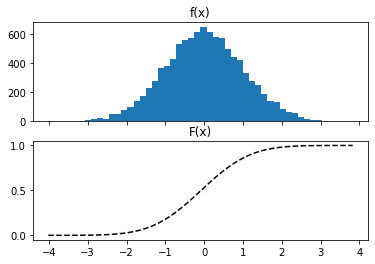
\includegraphics[width=8cm]{figs/PdfCdf}
\caption{\label{fig:PdfCdf} Probability distribution function $f(x)$ and cumulative distribution function of a normal distribution $F(x)$.}
\end{center}
\end{figure}

We can then interpret the CDF as a new variable $s = F(t)$, meaning that $F$ becomes a transformation that maps $t$ to $s$, i.e. $F:t \to s$. Accordingly,  $\lim_{t \to -\infty}s(t) = 0$ and $\lim_{t \to \infty}s(t) = 1$ and $s$ can be intuitively interpreted as the fraction of the distribution of $t$ with values smaller than $t$ from the definition of the CDF. This implies that the probability distribution of $s$, $g(s)$, is constant in the interval $s \in [0,1]$ in which $s$ is defined, and $s$ can be interpreted as the cumulative distribution of its own probability distribution:

\begin{equation}
s = G(s) = \int_{-\infty}^{s} g(s^\prime) ds^\prime
\end{equation}

In case of discrete probability functions, such as the negative binomial function, the same argument still holds, but the definition of the quantile function is replaced by the generalized inverse: $F^{-1}(y) = \mathrm{\inf \left \{x : F(x)>y\right  \} }$ for $y \in [0,1]$, see e.g. \cite[p. 54]{casella2002statistical}. In order to obtain a uniform distribution for discrete PDFs that is comparable to the case of continuous distributions, the histogram holding the values of the CDF is filled using random numbers according to the intervals of the CDF. For example, if the sales of zero items accounts for 75 percent of the observed sales distribution for this item, the value of the CDF function that is used to fill the histogram in case of zero actual sales is randomly chosen in the interval $[0, 0.75]$. Proceeding similarly for all other observed values, with the intervals from which to randomly choose values to fill in the histogram defined by the CDF values of the corresponding discrete sales value and the one below (e.g. for 3 actual sales: random pick between discrete CDF values for 2 and 3), the resulting histogram of CDF values is again uniform, as in the case of a continuous PDF.

A histogram of the actually observed CDF values for each individual PDF prediction (see \fig \ref{fig:pdf_example} for an example) is therefore expected to be uniformly distributed in $[0,1]$, if the predicted probability distribution $f(x)$ is correctly calibrated. This is illustrated in \fig \ref{fig:cdf_histos}, which shows the distribution of observed CDF values for five different cases. If both the choice of the model and the model parameters are estimated correctly, we would expect the uniform distribution. If the mean or the variance are not estimated correctly, the resulting distribution will show a distinct deviation from this uniform behavior.

\begin{figure}
\begin{center}
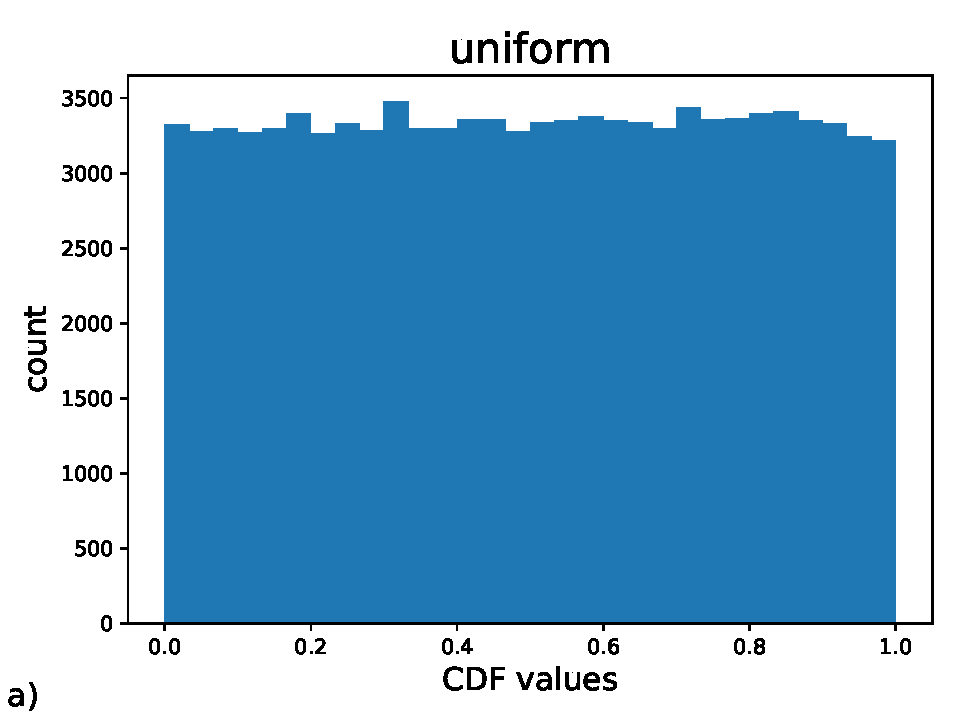
\includegraphics[scale=0.25]{figs/cdf_truth_uniform}
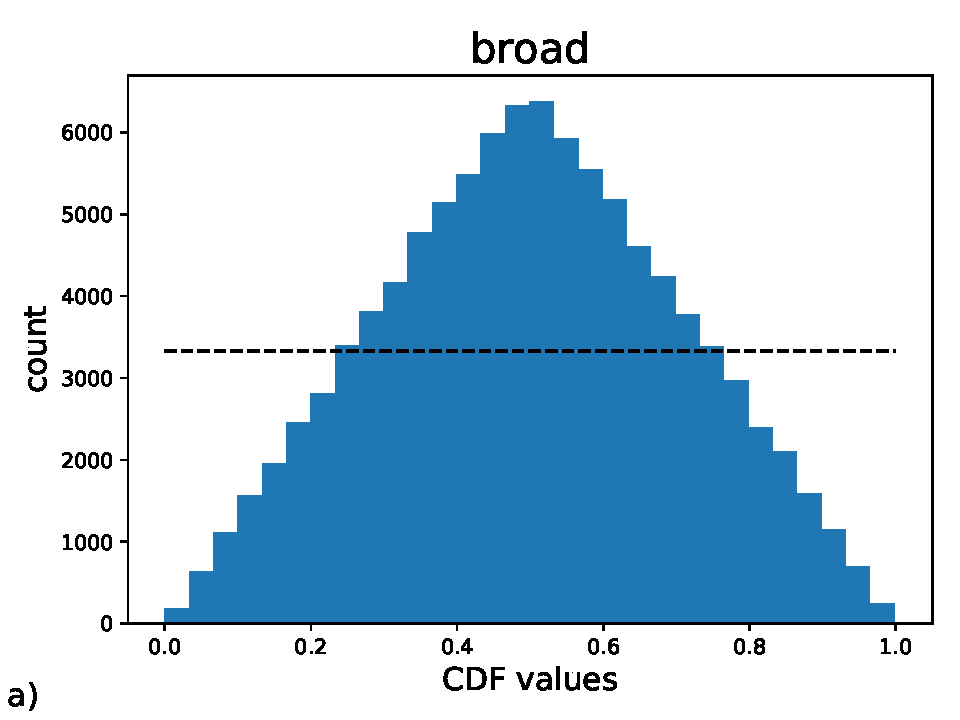
\includegraphics[scale=0.25]{figs/cdf_truth_broad}
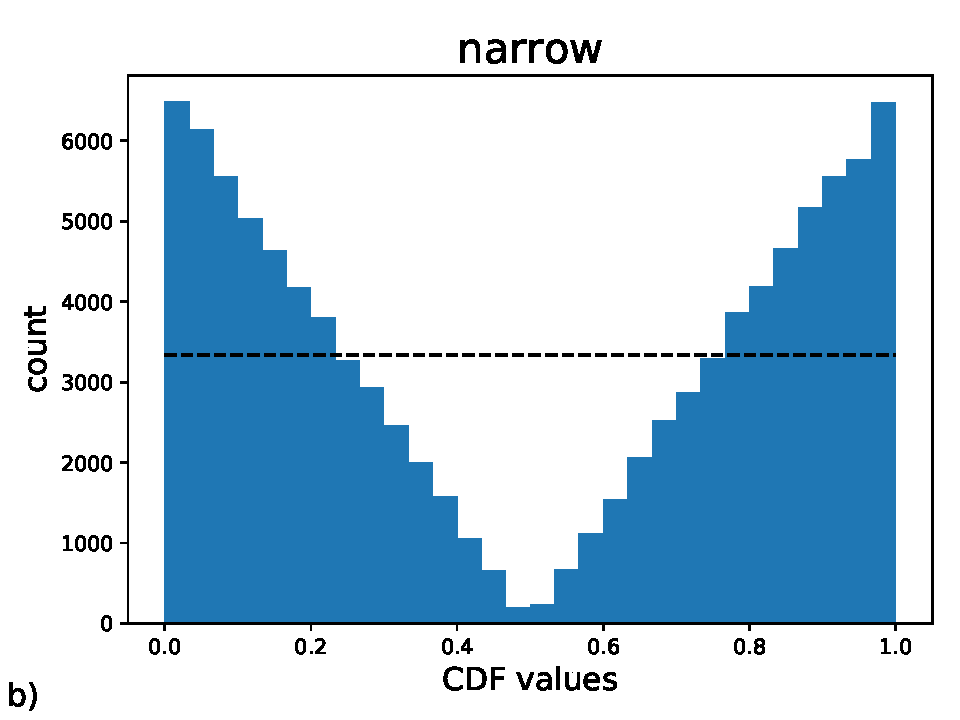
\includegraphics[scale=0.25]{figs/cdf_truth_narrow}
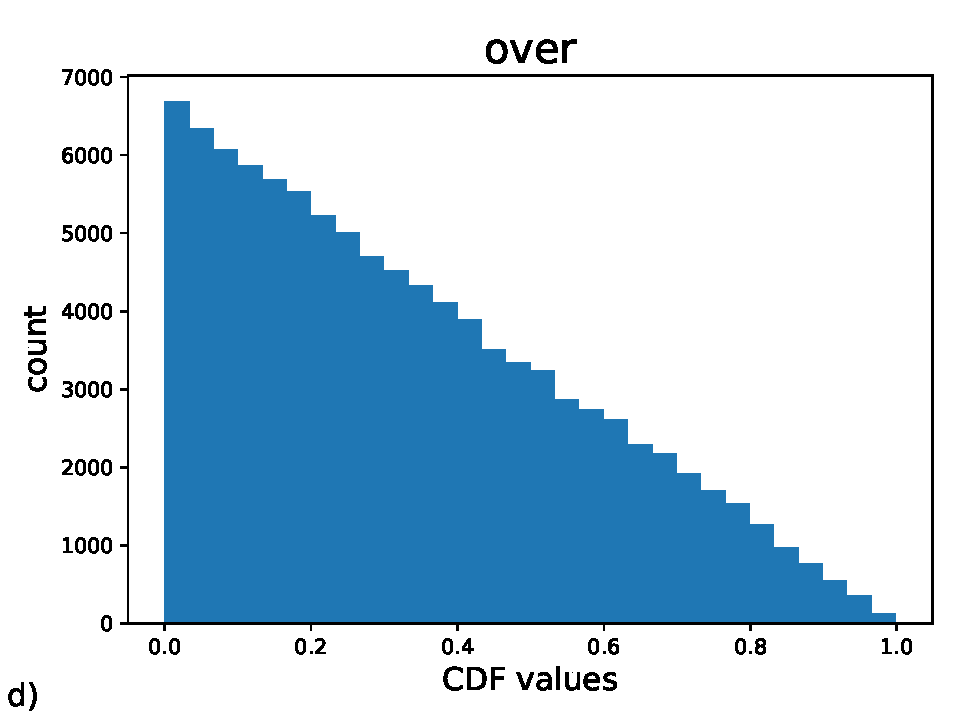
\includegraphics[scale=0.25]{figs/cdf_truth_over}
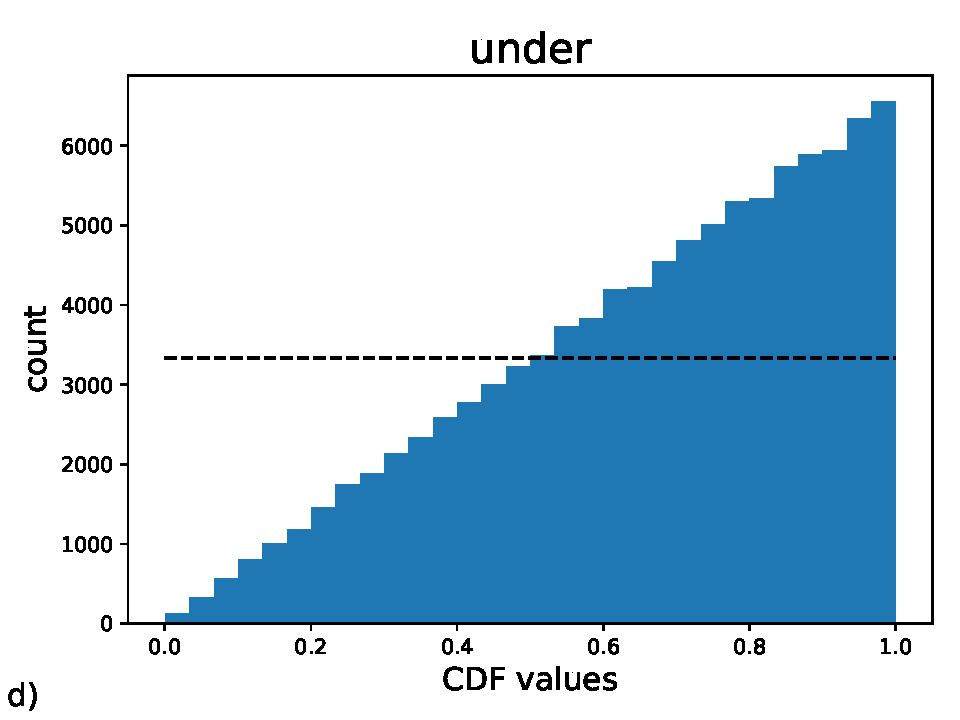
\includegraphics[scale=0.25]{figs/cdf_truth_under}
\caption{\label{fig:cdf_histos} Histogram of actually observed CDF values for different cases of estimating the full PDF compared to the expected uniform distribution:
correct prediction (a: ``uniform''), variance overestimated (b: ``broad''), variance underestimated (c: ``narrow''), mean overestimated (d: ``over''), mean underestimated (e: ``under'')}
\end{center}
\end{figure}

\noindent
It should be noted that the method requires a sufficient sample size, as a too low number of observations of course leads to a discretization bias.

\subsubsection{Inverse Quantile Profile Plot}

We now refine the method from sec. \ref{sec:cdf_histo} by comparing (in the sense of higher or lower) the CDF values of the observed events, i.e., the sales records, with specified quantiles. In order to do so, we start again from the predicted values for the mean and variance from which a negative binomial distribution is constructed for each prediction, for example, for the predicted demand for a single product sold on a single day in a given sales location. Each of these predicted negative binomial PDFs is then transformed to its CDF. Note that for simplicity, we always refer to the negative binomial model in this description, however, the general approach is valid for any PDF.

Then we compare the actual observed sales value (corrected for censored data if necessary) to different quantiles of the corresponding predicted distribution for each data record and average over a larger data sample. For example, if we wanted to check that the median of the distribution, corresponding to the quantile $0.5$, is predicted correctly by the machine learning model, we would compare the value $0.5$ to the ratio of CDF values (again randomly chosen from the corresponding range of CDF values for discrete target values, as described in sec. \ref{sec:cdf_histo}) of observed sales records being lower/higher than $0.5$. In other words, in case of the median, 50 percent of the ex post observed target values should be observed below the median of the corresponding individual predicted PDF and 50 percent above.

In order to judge whether the overall shape of the predicted distributions is predicted correctly, we repeat this procedure for a range of quantiles, for example $q = 0.1, 0.2, \ldots, 0.9$. However, we are free to choose which quantiles to look at, and in specific situations it might be advisable to look at the tails of the distribution in more detail, to make sure that even relatively rare events are estimated correctly by the machine learning algorithm, and add more quantiles for comparison in the region between, say $q = 0.95$ and $q = 0.99$. In the following, we call this method {\em inverse quantile profile plot}. Profile plots are akin to scatter plots and described in more detail in appendix \ref{sec:profile}.

\fig \ref{fig:invquant_example} illustrates five different collections of inverse quantile profile plots (each collection comparing to 6 specified quantile values, namely $q = 0.1$, $q = 0.3$, $q = 0.5$, $q = 0.7$, $q = 0.9$, and $q = 0.97$), for separate sets of exemplary PDF estimations and observed data combinations. The dashed horizontal lines indicates the fraction we expect, i.e., the specified quantile value, if the predictions are correct. For example, for the median, the line at $q = 0.5$ indicates that  50 percent of all PDF prediction and observed data combinations in a given data set should fall above the line, and 50 percent should fall below the line. The observation of the number of samples, indicated with different markers, that do in fact fall above and below a particular line, then allows the evaluation of the accuracy of PDF estimations. In case that the PDFs are not estimated correctly, the fractions will deviate from their expected values and the corresponding profile plot allows to judge whether for example the tails of the predicted distribution describing rare events are particularly problematic.

\begin{figure}
\begin{center}
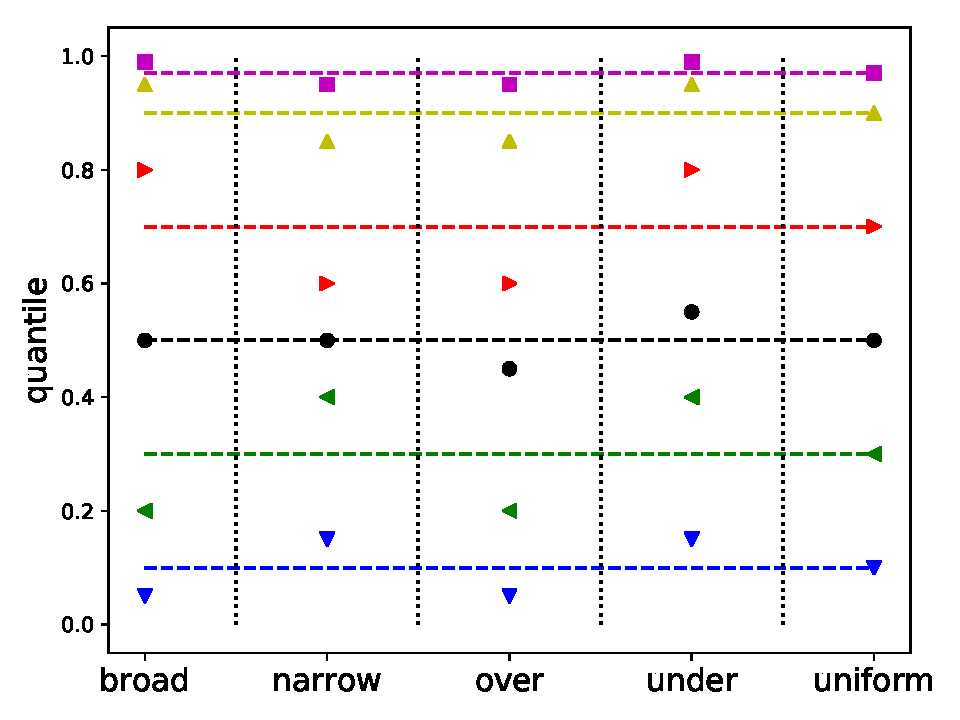
\includegraphics[width=8cm]{figs/invquant_example}
\caption{\label{fig:invquant_example} Five different inverse quantile profile plots (separated into columns by dotted vertical lines), each comparing all its predicted PDFs to the corresponding observed events. In the leftmost two columns, the outcome is illustrated if the estimate of the variance is biased, the center and center-right columns illustrate cases for which the mean estimation is biased, and the far right column shows the expected behavior if all predictions are correct.}
\end{center}
\end{figure}

In the same way as the method of filling all observed CDF values of the individual PDF predictions in a histogram and compare to a uniform distribution (described in sec. \ref{sec:cdf_histo}), inverse quantile profile plots do not work on individual PDF predictions but require a statistical population. However, calculating the fractions of the inverse quantile profile plots globally, i.e., over all samples in the data set, might not reveal certain deficiencies for a subset, e.g., a specific store or product group in the example of retail demand forecasts. Therefore, we combine the approach described above with the method of profile plots, where the quantity on the $x$-axis of the inverse quantile profile plot can be any variable of the data set at hand known at prediction time.

In summary, this approach has two major benefits compared to the method discussed in sec. \ref{sec:cdf_histo}: First, by explicitly visualizing several different quantiles, the inverse quantile profile plot reveals which part of the predicted PDF, such as the tails of the probability distribution, are particularly problematic. Second, by showing the dependency from the (arbitrary) variable on the $x$-axis, the inverse quantile profile plot reveals deviations of the predicted PDF from the actuals for different parts, e.g. specific categories, of that variable. Two examples for this can be found in Figs. \ref{fig:invquant_mean} and \ref{fig:invquant_dayofweek} in the next section.

\subsection{Quantitative Evaluation of PDF Predictions}
\label{sec:cdf_acc}

The methods discussed so far allow a detailed qualitative evaluation of PDF predictions. In order to also quantify the quality of the PDF predictions, we use a metric assessing the difference between two probability distributions to compare the histogram of CDF observations of the predicted PDFs with the expected uniform distribution, and define an accuracy measure in the range between 0 and 1, which takes the value of 1 when both distributions agree perfectly. Several approaches that measure the difference between two probability distributions are suggested in the literature, such as the first Wasserstein distance \cite{olkin1982}, also known as earth mover distance (EMD), the Kullback-Leibler divergence \cite{kullback1951}, also known as relative entropy, or the Jensen-Shannon divergence \cite{dagan1997}, also known as information radius.

Compared to the other mentioned methods, the first Wasserstein distance, representing the symmetric distance between two probability distributions on a given metric space, is more sensitive to smaller deviations, because it exhibits a linear behavior around zero (reflecting perfect agreement). Therefore, we focus on the first Wasserstein distance as the measure of difference in the following. For our purposes here, it can be defined by:
\begin{equation}
\text{EMD}(P, Q) = \frac{\sum_{k=1}^N |F_P(x_k) - F_Q(x_k)|}{N},
\end{equation}
where $F_P(X)$ and $F_Q(X)$ are the CDFs of the two PDFs $P(X)$ and $Q(X)$, respectively, and $x_k$ denotes the average value of $X$ in bin $k$, with $X$ being divided in $N$ bins.

Since $0.5$ represents the maximum value of the first Wasserstein distance when comparing any distribution in the support $[0, 1]$ to a flat distribution in the same interval (its minimum being zero), we define an accuracy measure for our PDF predictions in the range $[0, 1]$ by:
\begin{equation}
\text{accuracy} = 1 - 2 \cdot \text{EMD}
\end{equation}


\section{Example: Demand Forecasting}
\label{sec:example}

In the following, we describe how to use the approach outlined above in a practical setting. We use a public dataset obtained from a Kaggle online competition focusing in estimating unit sales of Walmart retail goods \cite{kaggle_data} for individual items for specific stores on specific days. For each demand forecast, Cyclic Boosting is used to predict the full probability density distribution of the expected demand at a granularity of (item, store, day) and use the methods described in sec. \ref{sec:pdfEvaluation} to evaluate the quality of the individual forecasts. Each data record corresponding to an observed sales record is described by the following fields: the identifier of an individual store store (\texttt{store\_id}), the product identifier (\texttt{item\_id}) as well as the date. The target $y$, that we need to predict, is the number of sales of a given product in a given store on a specific day, denoted by \texttt{sales}.

For our experiments, we use data from 2013-01-01 to 2016-05-22, that describe the sales of 100 different products (\texttt{FOODS\_3\_500}, ..., \texttt{FOODS\_3\_599}) of the department \texttt{FOODS\_3} in 10 stores.  All data before 2016 are used as the training data and the data from 2016 are used as an independent test or validation set. Besides the fields used to identify an individual sales record and the corresponding observed sales value, namely \texttt{item\_id}, \texttt{store\_id}, \texttt{date}, \texttt{sales}, we also use the fields \texttt{event\_name\_1}, \texttt{event\_type\_1}, \texttt{snap\_CA}, \texttt{snap\_TX}, \texttt{snap\_WI}, \texttt{sell\_price}, and \texttt{list\_price} in the forecasts and multiple features are built from these variables that are then used in the machine learning models.

\subsection{Mean Estimation}
\label{sec:example_mean}

As discussed earlier, we assume that each individual sale can be described by a Poisson-like process and we assume a negative binomial distribution to model the individual probability distribution of each sales event. As a first step, we use Cyclic Boosting (as described in sec. \ref{sec:CB}) to predict the mean of the distribution.

\noindent
This model uses the following variables as features: categorical variables for \texttt{store\_id} and \texttt{item\_id}, several derived variables that are constructed from the time-series of the sales records describing trend and seasonality (days since beginning of 2013 as linear trend as well as day of week, day of year, month, and week of month), time windows around the events given in the data set (7 days before until 3 days after for Christmas and Easter, and 3 days before until 1 day after for all other events like New Year or Thanksgiving), a flag denoting a promotion, and the ratio of reduced (\texttt{sell\_price}) and normal price (\texttt{list\_price}). We also include various two-dimensional combinations of these features. In these cases, one of the two dimensions is either \texttt{store\_id} or \texttt{item\_id}, allowing the machine learning model to learn characteristics of individual locations and products.

Unlike most state-of-the-art time series forecasting methods, we do not include lagged target information, for example via stacking of exponentially weighted moving average features, in our model. Although common in practice, including such variables makes the learning of exogenous effects, such as product promotions or the occurrence of special events, much harder. This is because when those variables are included, machine learning models tend to rely mainly on temporal confounding. Therefore, omitting these kind of variables improves the capability of the machine learning model to learn causal dependencies, which in turn improves the explainability of the model as well as the quality of the forecasts for mid- to long-term predictions and rare events. In order to capture recent trends that are not reflected in the exogenous features of the model, we apply an individual residual correction on each of the predictions of the machine learning model, which accounts for deviations between the exponentially weighted moving average (with a recursive smoothing factor of $0.15$) of the predictions and targets of each product-location combination over the corresponding past. We use the model to predict the expected demand two days into the future to reflect a realistic replenishment scenario, meaning that we use a target lag of two days for the training.

\noindent
We use the mean absolute deviation (MAD) as well as the mean squared error (MSE) as two common metrics for the evaluation of point estimates to give a rough estimate of the accuracy of the predicted mean. These metrics do not take the shape of the underlying probability distribution into account, but only compare the predicted mean to the observed number of sales. Using the independent test data, we obtain the following metrics: MAD: $1.65$ and MSE: $10.09$. The mean of the target, i.e. the observed sales, is $3.28$ for this period. \fig \ref{fig:mean_prediction} shows the time series of both predictions and sales summed over all 100 products and 10 stores during the test period.

\begin{figure}
\begin{center}
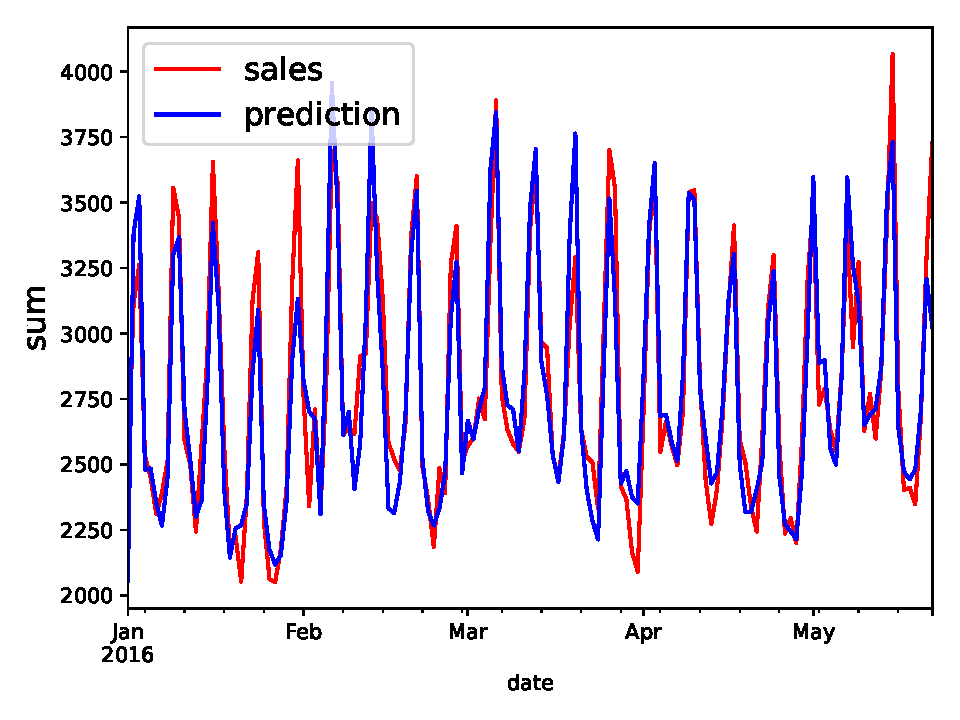
\includegraphics[width=8cm]{figs/ts_full}
\caption{\label{fig:mean_prediction} Time series of mean predictions and sales in test period summed over all products and stores.}
\end{center}
\end{figure}

\subsection{Variance Estimation}

The second model, based on Cyclic Boosting in its negative binomial width mode described in sec. \ref{sec:cb_width}, is used to estimate the variance of the negative binomial distribution. The data are split into training and test set as above and in addition the mean predictions for each individual product-location-date combination are fixed in the variance model as stated by \eqn \eqref{eqn:loss_likelihood}. This effectively means that the mean predictions are created in-sample for the training period using the fully trained and validated model for the mean discussed above.

\noindent
In this model focusing on the variance, we use the same set of features as for the mean model described above in sec. \ref{sec:example_mean}, except for dropping most of the two-dimensional combinations (only keeping \texttt{item\_id} - \texttt{store\_id}, \texttt{store\_id} - day of week, and \texttt{item\_id} - event type features) and adding the in-sample mean prediction as feature. An example for the resulting PDF and CDF predictions for item \texttt{FOODS\_3\_516} in store \texttt{TX\_3} on 2016-05-06, together with the corresponding observed sales value, is shown in \fig \ref{fig:pdf_example}.

\begin{figure}
\begin{center}
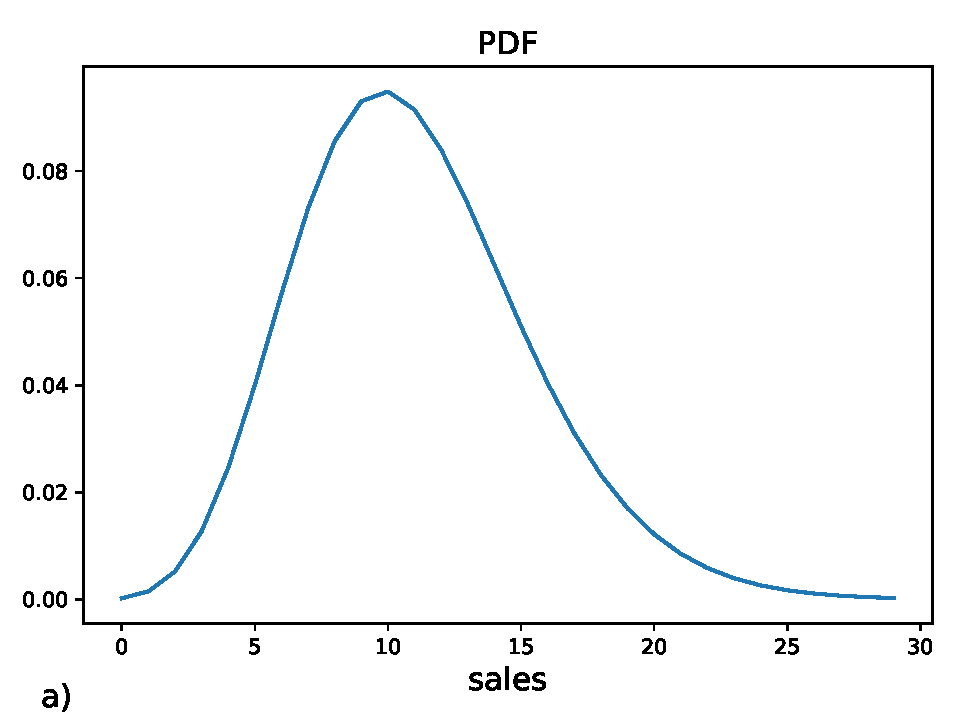
\includegraphics[width=4cm]{figs/pdf}
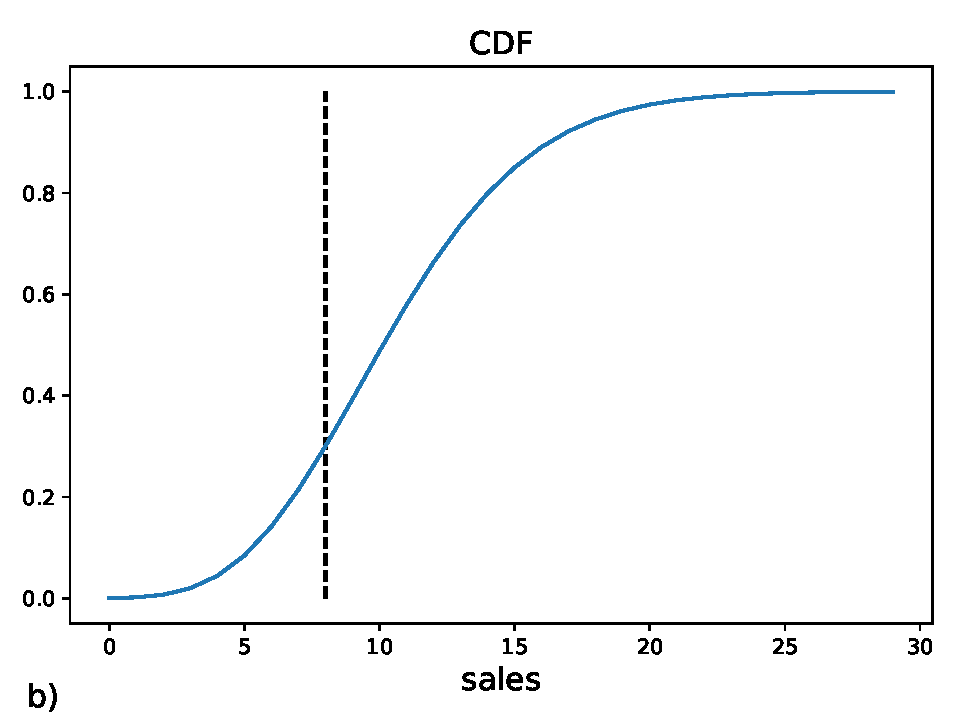
\includegraphics[width=4cm]{figs/cdf}
\caption{\label{fig:pdf_example} Predicted PDF (a) and CDF (b) for a specific product-location-date combination. The dashed vertical line in the CDF plot represents the actually observed sales, corresponding to a CDF value just under $0.3$.}
\end{center}
\end{figure}

\fig \ref{fig:factor_plots} visualizes the fully explainable nature of the individual Cyclic Boosting predictions, both for the mean and the variance model, by showing the time series plots of the factor values constituting the corresponding predictions for item \texttt{FOODS\_3\_516} in store \texttt{TX\_3} for all days in the test period from beginning of February to end of April 2016. Hereby, factors of different individual features, as described above, are multiplied, according to \eqn \eqref{eqn:cb} for the mean predictions and \eqn \eqref{eqn:r} for the variance predictions, in order to represent the behavior of a feature group. For example, the \texttt{events} feature group corresponds to the combination of all the factors of the different event features and the \texttt{dayofweek} feature group includes the one-dimensional feature \texttt{dayofweek} and its two-dimensional combinations with \texttt{store\_id} and \texttt{item\_id}.

\noindent
The different \texttt{item\_store} values for mean (higher than $1$) and variance model factors (lower than $1$), including the static one-dimensional features \texttt{store\_id} and \texttt{item\_id} and their two-dimensional combination, represent the fact that this product-location combination sells more than the average of all product-location combinations, and the dispersion parameter $1/r$ in \eqn \eqref{eqn:variance_r} in turn tends towards lower values. The explanation of the model for the peak in sales and mean prediction on February 7, 2016 is the event Super Bowl. The variance prediction for this day is driven by two competing factors:  the Super Bowl event itself drives  the  higher dispersion parameter higher, and the high mean prediction drives the lower dispersion parameter lower.

\begin{figure}
\begin{center}
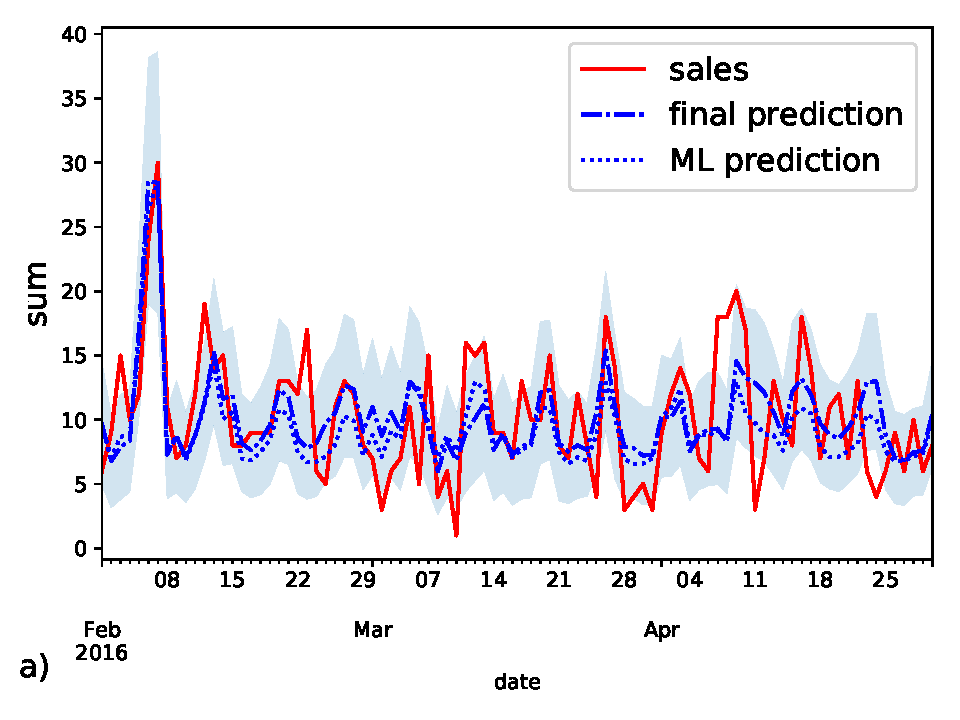
\includegraphics[width=4cm]{figs/ts_item_16_store_6}
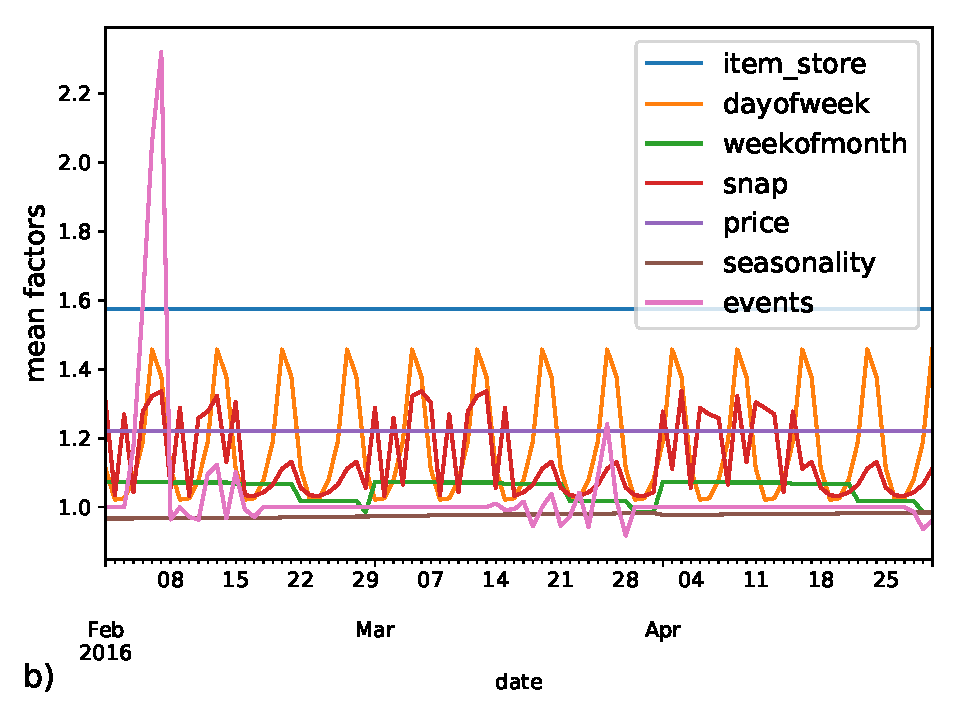
\includegraphics[width=4cm]{figs/factors_ts}
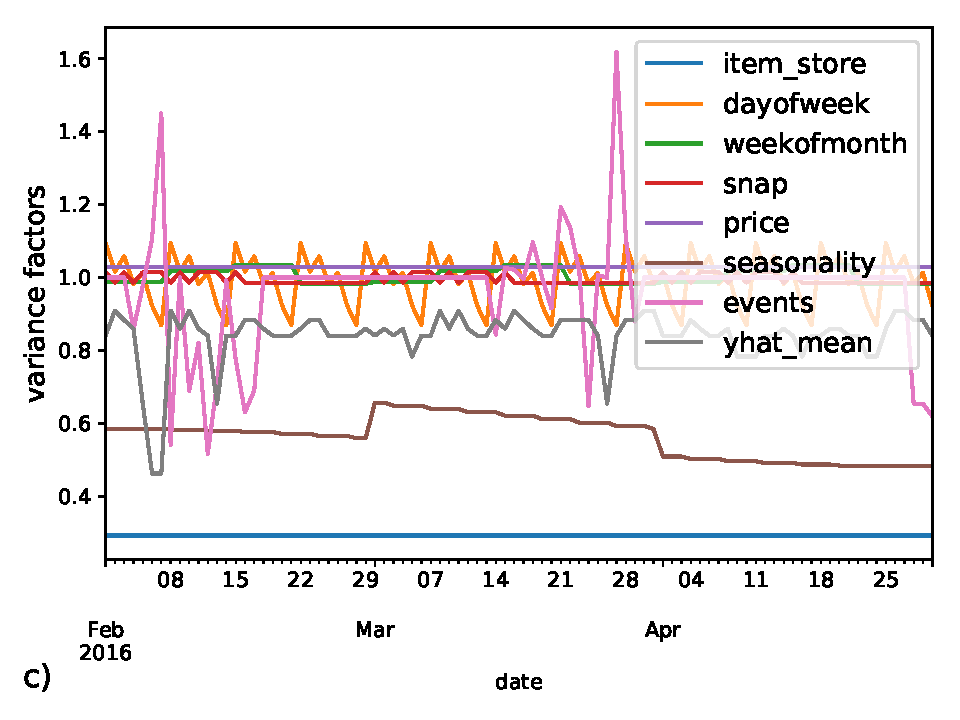
\includegraphics[width=4cm]{figs/factors_ts_width}
\caption{\label{fig:factor_plots} Time series of mean predictions (with the surrounding transparent band simplistically indicating a standard deviation as square root of the corresponding variance predictions) and sales (a), constituting factors of the mean predictions (b), and constituting factors of the variance predictions (c), for a specific product-location combination from beginning of February to end of April 2016. For both mean and variance predictions, the most granular constituting factors are aggregated, i.e. multiplied, for the sake of visualization.}
\end{center}
\end{figure}

\subsection{Evaluation of PDF Predictions}

\fig \ref{fig:cdf_demand} shows the histogram of CDF observations according to the method described in sec. \ref{sec:cdf_histo} for all product-location-day combinations in the test period. As benchmark, we compare the outcome of our negative binomial model to a simpler Poisson assumption, which has only a single model parameter, the mean. Using the same mean predictions for both negative binomial and Poisson model, the negative binomial PDF predictions are much closer to the uniform distribution, which we expect for optimal PDF predictions, than the Poisson PDF predictions, showing the effectiveness of our variance estimation.

\noindent
While the Poisson histogram shows a clear pattern of too narrow PDF predictions (see \fig \ref{fig:cdf_histos}), the most significant deviations of the negative binomial histogram from the uniform distribution can be found in the first bins of CDF values close to $0$ (overprediction) as well as in the last bins of CDF values close to $1$ (underprediction). The first case is mainly due to a slight zero-inflation of actual sales. The latter case primarily stems from slow moving articles with less than one item sold per store per day on average, what can be seen in plots c and d of \fig \ref{fig:cdf_demand}, where the spike at CDF values close to $1$ is reduced by excluding all samples with mean predictions lower than $1.0$. The resulting distribution for the negative binomial model indicates a slight tendency towards too broad PDF predictions, at least for some observations.

\begin{figure}
\begin{center}
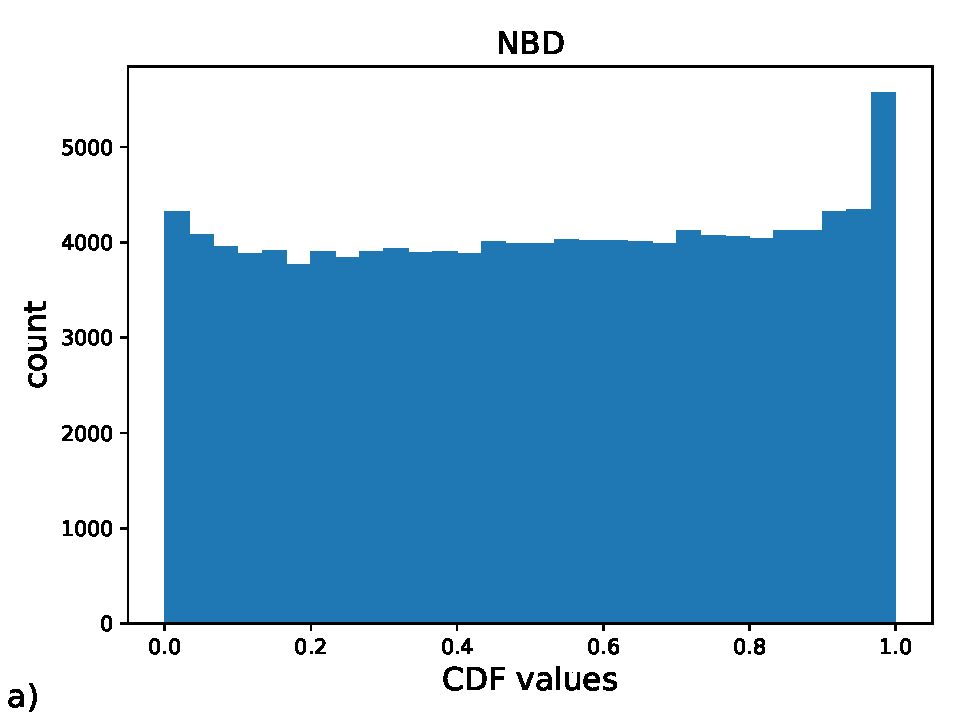
\includegraphics[width=4cm]{figs/cdf_truth_nbinom}
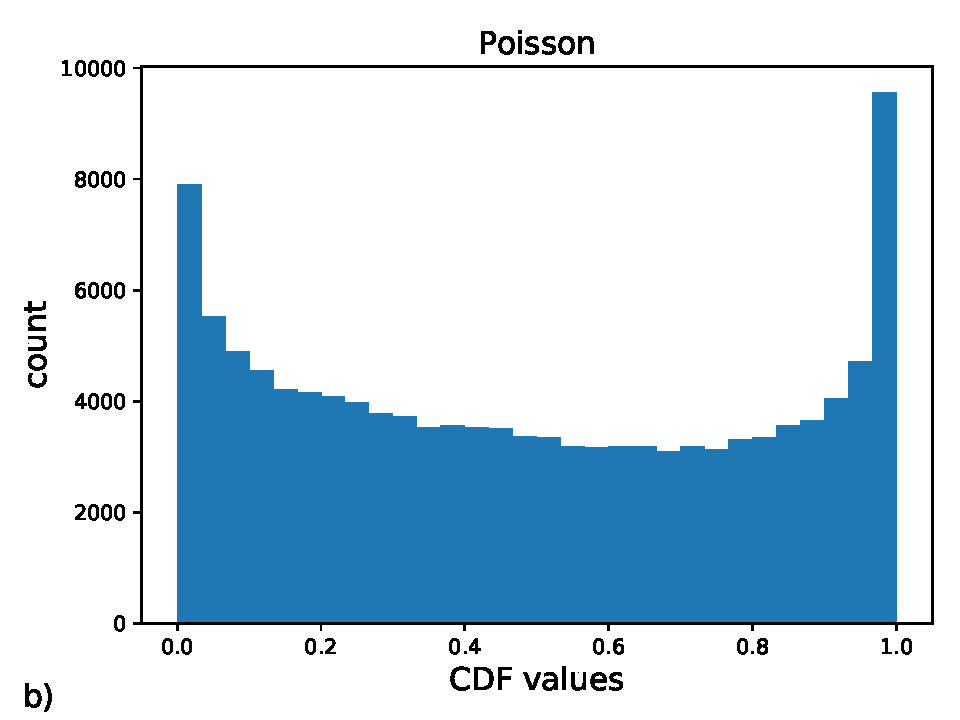
\includegraphics[width=4cm]{figs/cdf_truth_poisson}
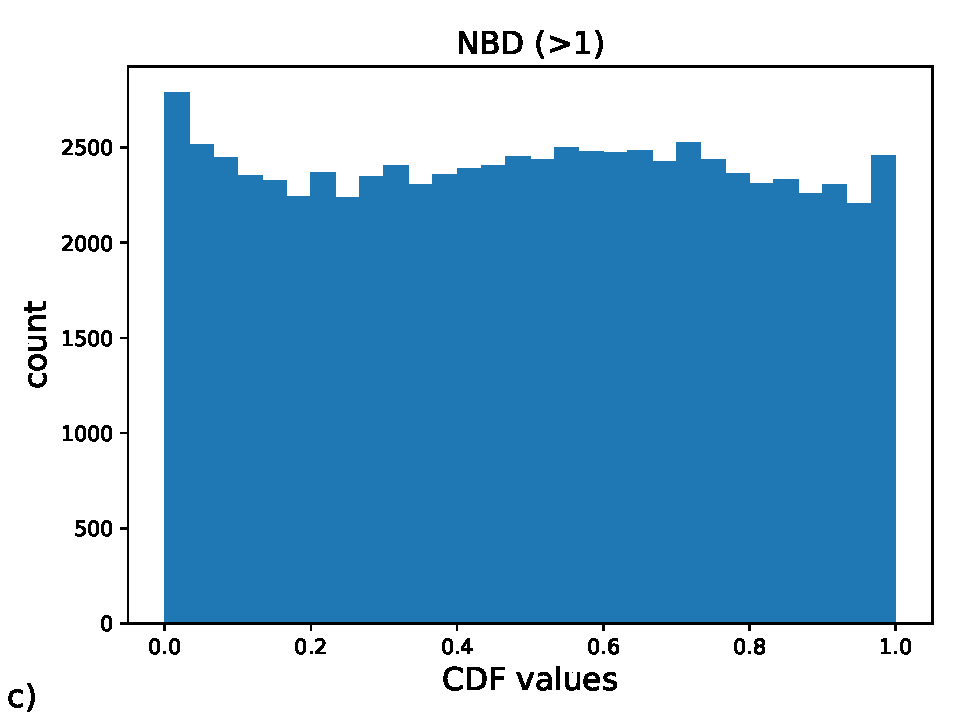
\includegraphics[width=4cm]{figs/cdf_truth_nbinom_larger1}
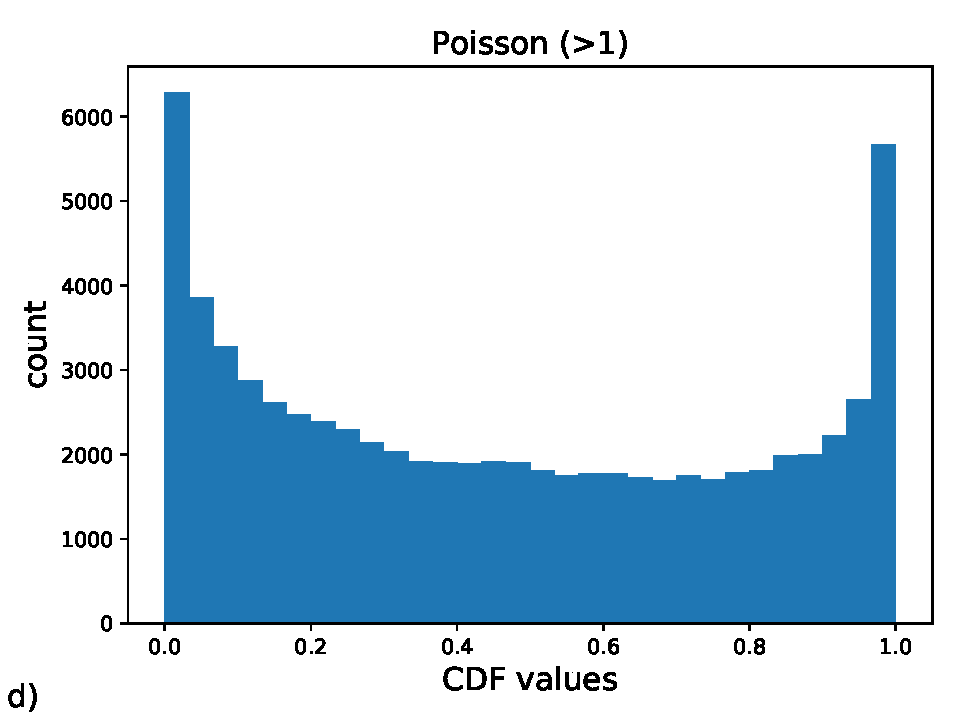
\includegraphics[width=4cm]{figs/cdf_truth_poisson_larger1}
\caption{\label{fig:cdf_demand} Histograms of ex post observed target CDF values of the corresponding individual PDF predictions (to be compared to a uniform distribution) for our negative binomial model (a) and a simpler Poisson model for comparison (b), using all product-location-day combinations in the test period. In order to show the effect of slow-sellers, both negative binomial (c) and Poisson model (d) histograms are also shown using samples with mean predictions higher than $1.0$ only.}
\end{center}
\end{figure}

Using the inverse quantile profile plots introduced earlier, the prediction quality of the full predicted PDF can be assessed in more detail. In \fig \ref{fig:invquant_dayofweek}, each column corresponds to a day of the week, using 0 for Mondays, 1 for Tuesdays, etc., and the considered quantiles are 0.1, 0.3, 0.5, 0.7, 0.9, and 0.97. Again, we compare the outcome of our negative binomial model to a simpler Poisson assumption. Aggregating over all stores, items, and sales dates (independently for each day of the week), we can see that for the negative binomial model each quantile is predicted relatively well, except for Sundays showing a tendency for overprediction of the mean (see \fig \ref{fig:invquant_example}). The Poisson model, on the other hand, shows a significant pattern of too narrow PDF predictions across all days of the week.

\begin{figure}
\begin{center}
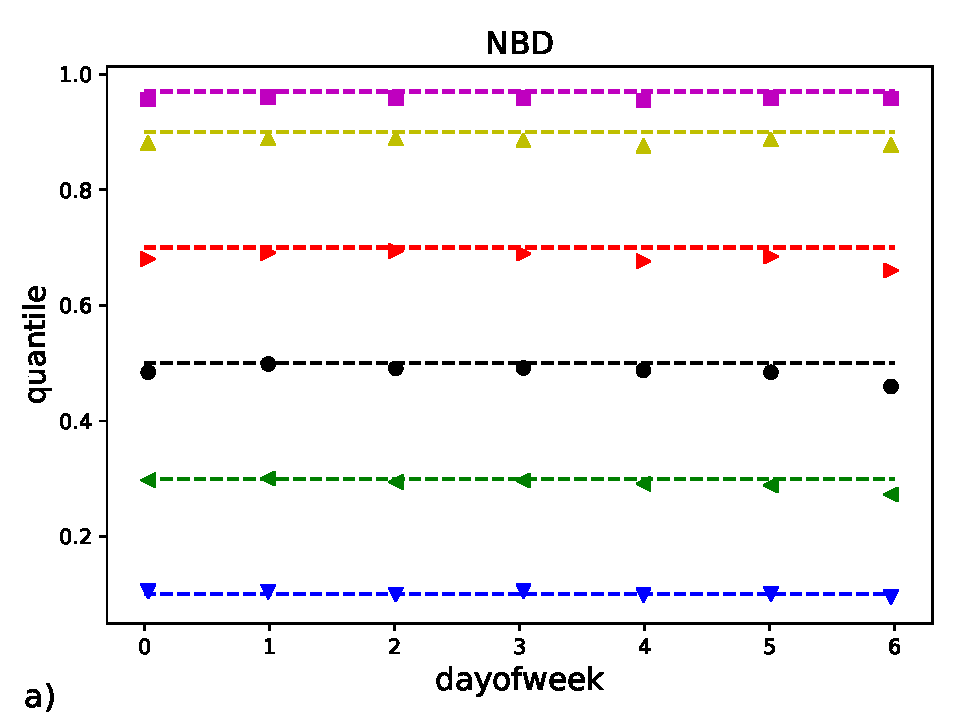
\includegraphics[width=4cm]{figs/invquant_dayofweek_nbinom}
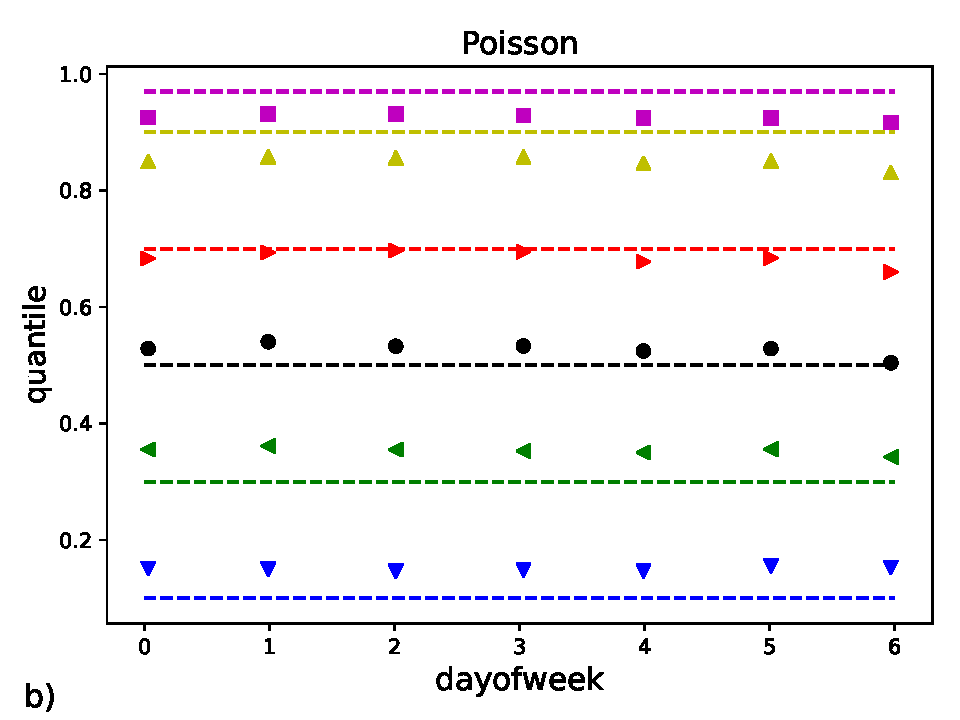
\includegraphics[width=4cm]{figs/invquant_dayofweek_poisson}
\caption{\label{fig:invquant_dayofweek} Inverse quantile profile plot for the different days of week on the $x$-axis (from Monday to Sunday) aggregated over all product-location-day combinations in the test period, for our negative binomial model (a) and a simpler Poisson model for comparison (b).}
\end{center}
\end{figure}

\fig \ref{fig:invquant_mean} shows the inverse quantile profile plot using the predicted mean as the $x$-axis of the graph, meaning that the distributions are grouped such that the 15 columns correspond to mean predictions in 12 intervals with widths of 5 from 0.0 to 60.0 and 3 remaining intervals $[60.0, 70.0]$, $(70.0, 80.0]$, and $(80.0, 100.0]$ (with mean predictions higher than 100.0 included in the highest interval), while we aggregate over all locations, items, and sales dates. The considered quantiles are chosen to be the same as in \fig \ref{fig:invquant_dayofweek}. While the Poisson model again shows a significant pattern of too narrow PDF predictions across the full range of mean prediction values, we can also see several deviations from the expected uniform behavior for the negative binomial model. For mean predictions around $30$, the negative binomial model deviates significantly from the expected behavior, with the shape of the deviations pointing towards too broad PDF predictions (as also observed in the CDF histogram above). And for mean predictions higher than $80$, the pattern of the deviations indicate an underprediction of the mean parameter. The deviations at very low predicted mean values reflect the complications of zero-inflation and slow-sellers seen in the first and last bins of the CDF histograms above.

\noindent
In a real-live situation with a live supply chain project for a customer, a more detailed investigation of the root-causes would then start. However, it should be noted that due to this segregation, the statistics in each part of the relevant test sample becomes a limiting factor as well. This plot also illustrates the benefits of using the quantile profile plot, since we have seen that using more conventional approaches, such as \fig \ref{fig:mean_prediction} or even the lower part of \fig \ref{fig:cdf_demand}, the predictions appear reasonable, even when not relying on simple point metrics such as MAD or MSE. It is therefore paramount both to predict the full probability distribution instead of just a point estimate, such as the mean, as well as verifying a number of quantiles for each prediction to assess the quality of the prediction thoroughly.

\begin{figure}
\begin{center}
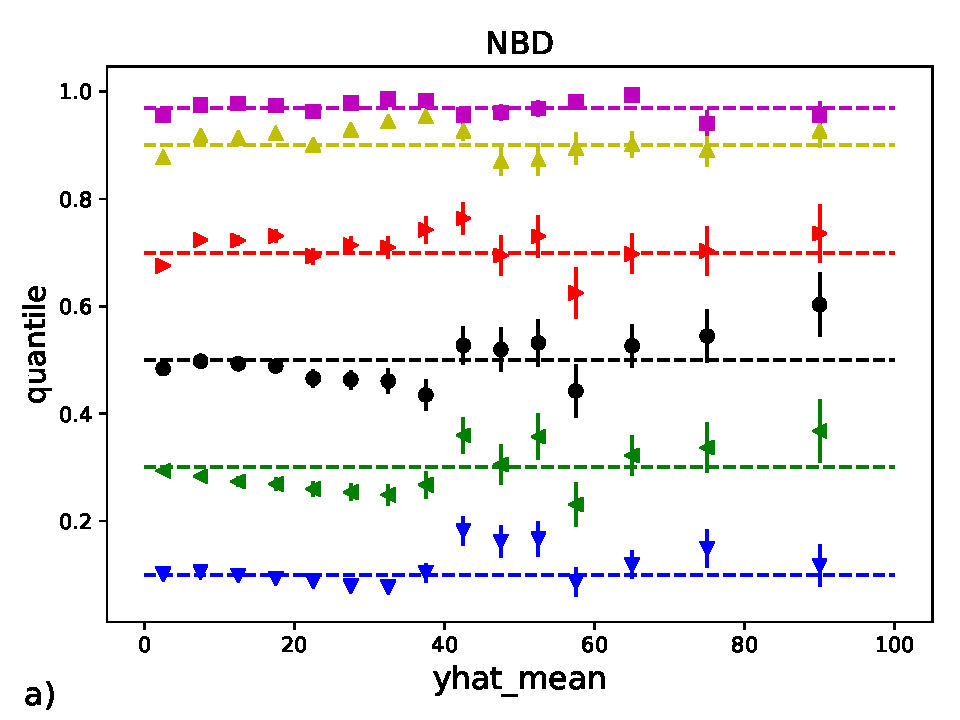
\includegraphics[width=4cm]{figs/invquant_yhat_mean_nbinom}
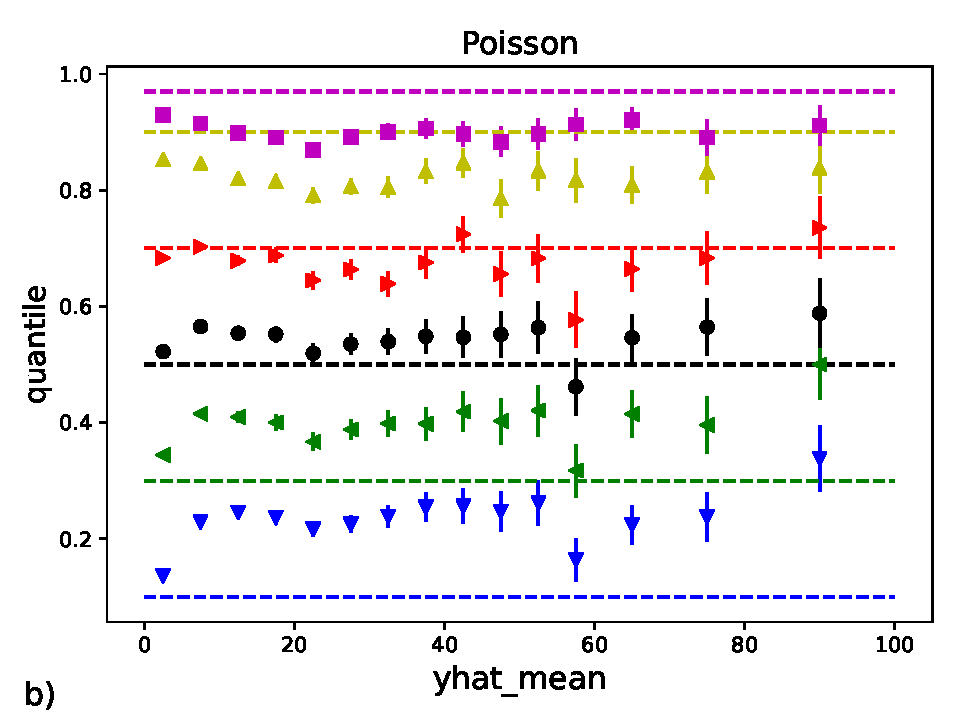
\includegraphics[width=4cm]{figs/invquant_yhat_mean_poisson}
\caption{\label{fig:invquant_mean} Inverse quantile profile plot for mean predictions on the $x$-axis aggregated over all product-location-day combinations in the test period, for our negative binomial model (a) and a simpler Poisson model for comparison (b).}
\end{center}
\end{figure}

The quantitative results for the CDF accuracy of our PDF predictions using the first Wasserstein distance as metric (as described in sec. \ref{sec:cdf_acc}) and calculated over all product-location-day combinations in the test period, can be found in \tab \ref{tab:cdf_acc}. As benchmark, we again compare against a Poisson model assumption using the same mean predictions. As expected from the qualitative findings in \fig \ref{fig:cdf_demand}, the negative binomial PDF predictions show a significant improvement over the simpler Poisson model.

\begin{table}[h!]
\begin{center}
\caption{Accuracy for negative binomial and Poisson PDF predictions, using the first Wasserstein distance as metric, calculated over all product-location-day combinations in the test period.}
\label{tab:cdf_acc}
\begin{tabular}{c|c|c}
 & \textbf{NBD} & \textbf{Poisson} \\
\hline
\textbf{EMD accuracy} & 0.967 & 0.850
\end{tabular}
\end{center}
\end{table}


\section{Conclusion}
Demand forecasting remains a crucial step in operational planning for retailers. Both from practical and theoretical perspectives, disentangling the forecast of demand from the operational decision making regarding order quantities has potentially significant advantages over an integrated approach using data to predict the resulting order quantities directly. When predicting future demand, both model-free and a model-based approaches can be used, where the model-based approach is generally more robust, as it is rooted in a theoretical understanding of the sales process. Compared to a model-free approach like quantile regression, the distributional assumption can drastically reduce the uncertainty of the resulting predictions. Using the Cyclic Boosting machine learning approach, the full probability density distribution can be predicted in a fully explainable way on the individual level. This allows to extract not only simple point estimates, such as the expected mean demand, but all relevant quantiles of the distribution.

Once the full probability density functions are forecasted, their evaluation poses significant challenges: Common metrics, such as the mean absolute deviation or mean squared error, only take point estimates into account and are generally not suitable for the evaluation of predicted probability distributions. Furthermore, since the distributions are predicted for individual events, statistical techniques aiming at the comparison of distributions using many events cannot be used in general. Instead, novel techniques exploiting the probability integral transform, namely the histogram of observed CDF values of the predicted individual PDFs as well as inverse quantile profile plots, allow a detailed investigation into the behavior of the predictions. Finally, a quantitative assessment resulting in a single number can be obtained using metrics such as the earth mover distance in a comparison between the histogram of observed CDF values and the expected uniform distribution.


% Authors must disclose all relationships or interests that 
% could have direct or potential influence or impart bias on 
% the work: 
%
%\section*{Declarations}
%
%\subsection*{Funding}
%No external funding was obtained for this work.
%
%\subsection*{Conflict of interest}
%
%\noindent
%Authors Felix Wick and Michael Feindt applied for a US patent ``A System and Method of Cyclic Boosting for Explainable Supervised Machine Learning''.
%
%\noindent
%Authors Felix Wick, Martin Hahn, and Moritz Wolf applied for a US patent ``Causal Factor Machine Learning with Individual Negative Binomial Probability Density Function Estimation''.
%
%\noindent
%Authors Felix Wick and Trapti Singhal applied for a US patent ``Evaluation of Predictions as Individual Probability Density Functions''.
%
%
%\subsection*{Availability of data and material}
%Data used in this work are public \cite{kaggle_data}
%
%\subsection*{Code availability}
%The details of the code are available from \cite{Wick2019}
%
%\subsection*{Authors' contributions}
%F. Wick: Code examples and manuscript text, U. Kerzel: manuscript text, M. Hahn, M. Wolf, T. Singhal, M. Feindt: revision 

\bibliography{paper}

% Springer
%\bibliographystyle{spmpsci}      % mathematics and physical sciences
\bibliographystyle{ieeetr}

%%
%% Appendices
%%
\appendix

\section{Profile Histograms}
\label{sec:profile}

In many cases, scatter plots are used to study the behavior of two distributions or sets of data points visually. However, even for moderate amount of data, this approach quickly becomes difficult. To illustrate this, a sample of $(x,y)$ data points was obtained in the following way: The distribution of $x$ values was obtained by generating 5,000 samples of Gaussian distributed random numbers $X \sim {\cal N}(0.0,2.0)$ and the $y$ values are obtained via $Y \sim X +  {\cal N}(2.0,1.5)$. \fig \ref{fig:scatter} shows the marginal distributions for $x$ and $y$ as well as a scatter plot of $x$ vs. $y$.

\begin{figure}
\begin{center}
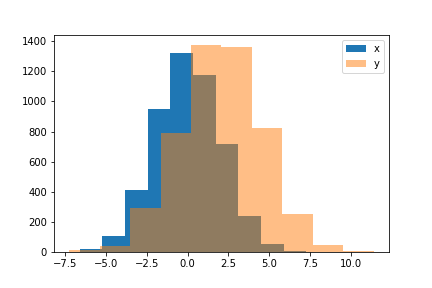
\includegraphics[scale=0.5]{figs/marginal} 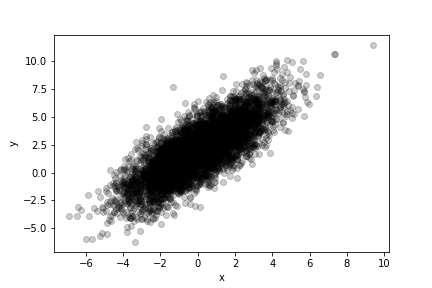
\includegraphics[scale=0.5]{figs/scatter}
\caption{\label{fig:scatter} Marginal distribution and scatter plot of variables $X$ and $Y$.}
\end{center}
\end{figure}

Although the simple linear correlation between $X$ and $Y$ is apparent in the scatter plot, finer details are not visible and it is easy to imagine that a more complex relationship is difficult to discern. Profile histograms are specifically designed to address this shortcoming. Intuitively, profile histograms are a one-dimensional representation of the two-dimensional scatter plot and are obtained  in the following way: The variable on the $x$ axis is discretized into a suitable range of bins. The exact choice of binning depends on the problem at hand. One can for example choose equidistant bins in the range of the $x$ axis or non-equidistant bins such that each bin contains the same number of observations. Then within each bin of the variable $X$, the a location and dispersion metric is calculated for the variable $Y$. This means that the bin-borders on the $X$ axis are used as constraints on the variable $Y$ and with these conditions applied, for example the sample mean of the selected $y$ values as well as the standard deviation are calculated. These location and dispersion metrics in each bin of $X$ are used to illustrate the behavior of the variable $Y$ as the values of the variable $X$ change from bin to bin. The resulting profile histogram is shown in \fig \ref{fig:profile}. This one-dimensional representation allows to understand even a complex relationship between two variables visually. Note that due to few data points at the edges of the distributions the profile histogram is expected to show visual artifacts in the corresponding regions.

 \begin{figure}
\begin{center}
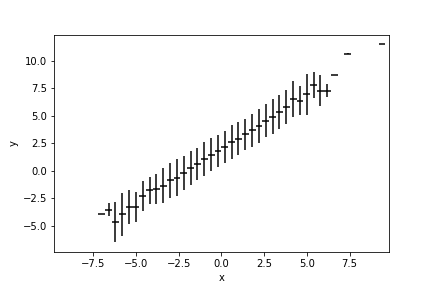
\includegraphics[scale=0.5]{figs/profile}
\caption{\label{fig:profile} Profile histogram of variables $X$ and $Y$.}
\end{center}
\end{figure}


\end{document}
